\documentclass[tikz, border=10pt]{standalone}
\usepackage{newtxtext,newtxmath}
\usetikzlibrary{arrows.meta, shapes.geometric, fit, positioning, calc, backgrounds}

\definecolor{steelblue}{HTML}{576fa0}
\definecolor{steelbluelight}{HTML}{a7b9d7}
\definecolor{gold}{HTML}{e3b87f}
\definecolor{goldlight}{HTML}{fadcb4}
\definecolor{rose}{HTML}{b57979}
\definecolor{roselight}{HTML}{dea3a2}
\definecolor{morandigray}{HTML}{9f9f9f}
\definecolor{morandigraylight}{HTML}{cfcece}
\definecolor{bgblue}{HTML}{e8edf5}
\definecolor{bggold}{HTML}{f5eedf}
\definecolor{bgrose}{HTML}{f0e2e2}
\definecolor{bggray}{HTML}{ececec}
\definecolor{bggreen}{HTML}{e2ede6}
\definecolor{indigo}{HTML}{6366F1}
\definecolor{indigolight}{HTML}{c7d2fe}
\definecolor{bgindigo}{HTML}{eef2ff}

\begin{document}
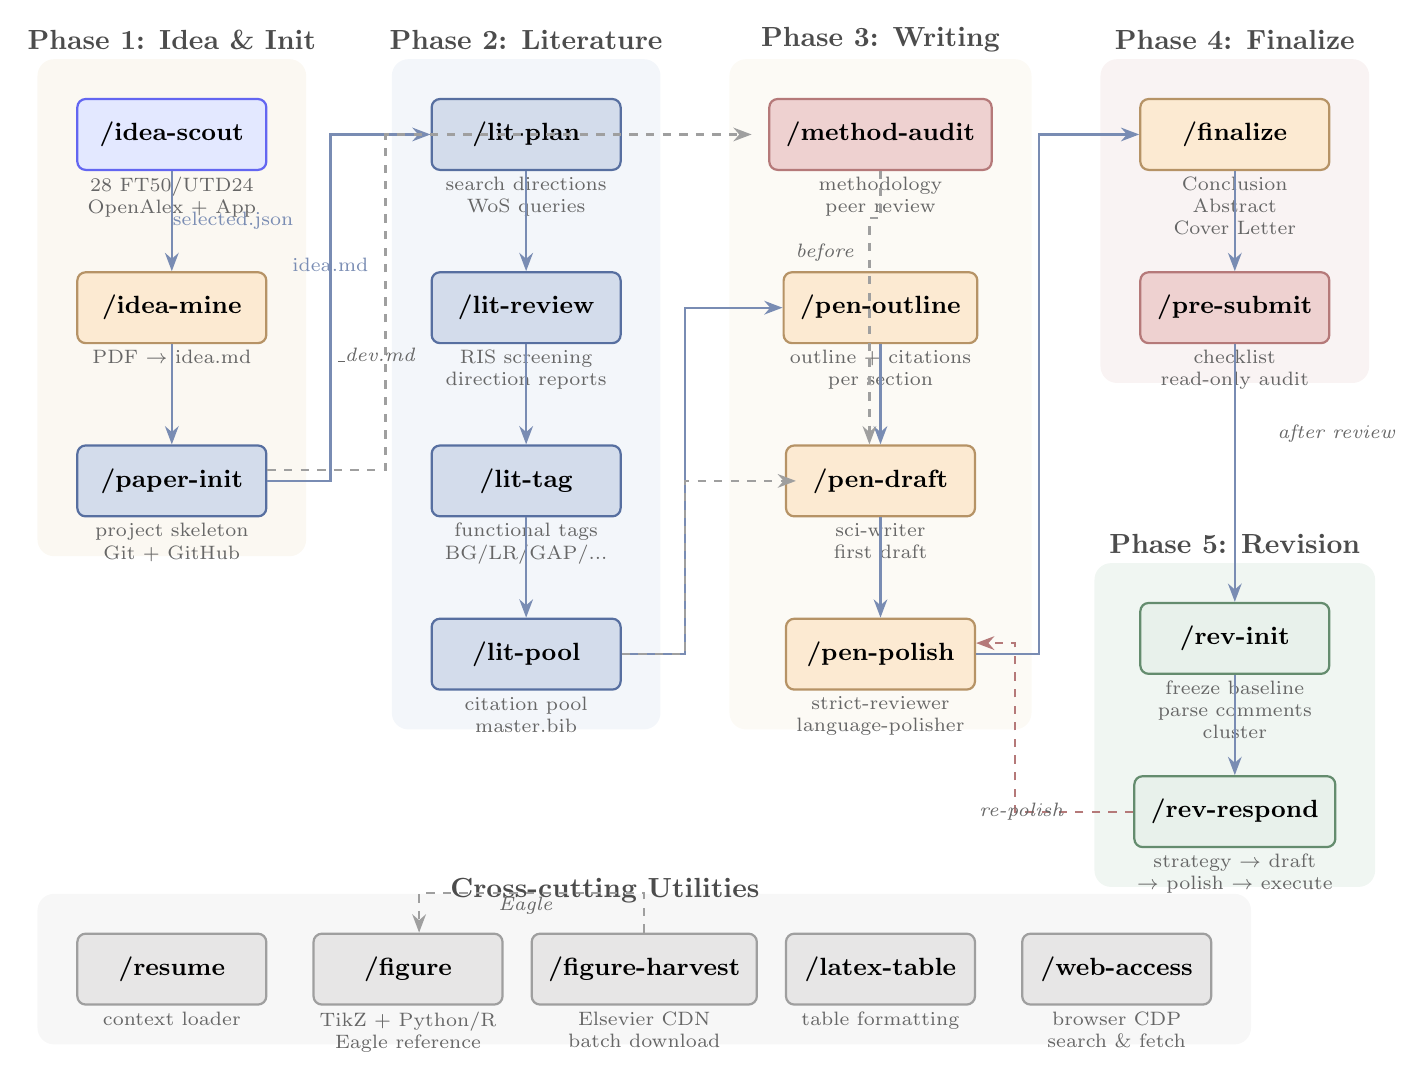
\begin{tikzpicture}[
  font=\small,
  >=Stealth,
  every node/.style={inner sep=0pt},
  skill/.style={
    draw=steelblue, thick, rectangle, rounded corners=3pt,
    fill=steelbluelight!50, align=center, inner sep=6pt,
    minimum width=2.4cm, minimum height=0.9cm,
    font=\small\bfseries,
  },
  skillgold/.style={
    draw=gold!80!black, thick, rectangle, rounded corners=3pt,
    fill=goldlight!60, align=center, inner sep=6pt,
    minimum width=2.4cm, minimum height=0.9cm,
    font=\small\bfseries,
  },
  skillrose/.style={
    draw=rose, thick, rectangle, rounded corners=3pt,
    fill=roselight!50, align=center, inner sep=6pt,
    minimum width=2.4cm, minimum height=0.9cm,
    font=\small\bfseries,
  },
  skillgray/.style={
    draw=morandigray, thick, rectangle, rounded corners=3pt,
    fill=morandigraylight!50, align=center, inner sep=6pt,
    minimum width=2.4cm, minimum height=0.9cm,
    font=\small\bfseries,
  },
  skillgreen/.style={
    draw={rgb,255:red,100;green,140;blue,110}, thick, rectangle, rounded corners=3pt,
    fill=bggreen!80, align=center, inner sep=6pt,
    minimum width=2.4cm, minimum height=0.9cm,
    font=\small\bfseries,
  },
  skillindigo/.style={
    draw=indigo, thick, rectangle, rounded corners=3pt,
    fill=indigolight!50, align=center, inner sep=6pt,
    minimum width=2.4cm, minimum height=0.9cm,
    font=\small\bfseries,
  },
  desc/.style={font=\scriptsize\color{black!60}, align=center},
  arr/.style={->, thick, steelblue!80},
  arrdash/.style={->, thick, dashed, morandigray},
  phase/.style={font=\normalsize\bfseries, text=black!70},
]

%% ============================================================
%% COLUMN 1: Idea & Init Phase (x=0)
%% ============================================================
\node[phase] at (0, 1.2) {Phase 1: Idea \& Init};

\node[skillindigo] (ideascout) at (0, 0) {/idea-scout};
\node[desc, below=2pt of ideascout] {28 FT50/UTD24\\OpenAlex + App};

\node[skillgold] (ideamine) at (0, -2.2) {/idea-mine};
\node[desc, below=2pt of ideamine] {PDF $\to$ idea.md};

\node[skill] (paperinit) at (0, -4.4) {/paper-init};
\node[desc, below=2pt of paperinit] {project skeleton\\Git + GitHub};

%% ============================================================
%% COLUMN 2: Literature Phase (x=4.5)
%% ============================================================
\node[phase] at (4.5, 1.2) {Phase 2: Literature};

\node[skill] (litplan) at (4.5, 0) {/lit-plan};
\node[desc, below=2pt of litplan] {search directions\\WoS queries};

\node[skill] (litreview) at (4.5, -2.2) {/lit-review};
\node[desc, below=2pt of litreview] {RIS screening\\direction reports};

\node[skill] (littag) at (4.5, -4.4) {/lit-tag};
\node[desc, below=2pt of littag] {functional tags\\BG/LR/GAP/...};

\node[skill] (litpool) at (4.5, -6.6) {/lit-pool};
\node[desc, below=2pt of litpool] {citation pool\\master.bib};

%% ============================================================
%% COLUMN 3: Writing Phase (x=9)
%% ============================================================
\node[phase] at (9, 1.2) {Phase 3: Writing};

\node[skillrose] (methodaudit) at (9, 0) {/method-audit};
\node[desc, below=2pt of methodaudit] {methodology\\peer review};

\node[skillgold] (penoutline) at (9, -2.2) {/pen-outline};
\node[desc, below=2pt of penoutline] {outline + citations\\per section};

\node[skillgold] (pendraft) at (9, -4.4) {/pen-draft};
\node[desc, below=2pt of pendraft] {sci-writer\\first draft};

\node[skillgold] (penpolish) at (9, -6.6) {/pen-polish};
\node[desc, below=2pt of penpolish] {strict-reviewer\\language-polisher};

%% ============================================================
%% COLUMN 4: Finalize Phase (x=13.5)
%% ============================================================
\node[phase] at (13.5, 1.2) {Phase 4: Finalize};

\node[skillgold] (finalize) at (13.5, 0) {/finalize};
\node[desc, below=2pt of finalize] {Conclusion\\Abstract\\Cover Letter};

\node[skillrose] (presubmit) at (13.5, -2.2) {/pre-submit};
\node[desc, below=2pt of presubmit] {checklist\\read-only audit};

%% ============================================================
%% COLUMN 5: Revision Phase (x=13.5, lower)
%% ============================================================
\node[phase] at (13.5, -5.2) {Phase 5: Revision};

\node[skillgreen] (revinit) at (13.5, -6.4) {/rev-init};
\node[desc, below=2pt of revinit] {freeze baseline\\parse comments\\cluster};

\node[skillgreen] (revrespond) at (13.5, -8.6) {/rev-respond};
\node[desc, below=2pt of revrespond] {strategy $\to$ draft\\$\to$ polish $\to$ execute};

%% ============================================================
%% CROSS-CUTTING: Utility Skills (bottom)
%% ============================================================
\node[phase] at (5.5, -9.6) {Cross-cutting Utilities};

\node[skillgray] (resume) at (0, -10.6) {/resume};
\node[desc, below=2pt of resume] {context loader};

\node[skillgray] (figure) at (3, -10.6) {/figure};
\node[desc, below=2pt of figure] {TikZ + Python/R\\Eagle reference};

\node[skillgray] (figharvest) at (6, -10.6) {/figure-harvest};
\node[desc, below=2pt of figharvest] {Elsevier CDN\\batch download};

\node[skillgray] (latextable) at (9, -10.6) {/latex-table};
\node[desc, below=2pt of latextable] {table formatting};

\node[skillgray] (webaccess) at (12, -10.6) {/web-access};
\node[desc, below=2pt of webaccess] {browser CDP\\search \& fetch};

%% ============================================================
%% ARROWS: Main Pipeline
%% ============================================================

% Phase 1 internal
\draw[arr] (ideascout) -- node[right, desc] {selected.json} (ideamine);
\draw[arr] (ideamine) -- (paperinit);

% Phase 1 -> Phase 2
\draw[arr] (paperinit.east) -- ++(0.8,0) |- node[above, desc, pos=0.3] {idea.md} (litplan.west);

% Phase 2 internal
\draw[arr] (litplan) -- (litreview);
\draw[arr] (litreview) -- (littag);
\draw[arr] (littag) -- (litpool);

% Phase 2 -> Phase 3
\draw[arr] (litpool.east) -- ++(0.8,0) |- (penoutline.west);

% Phase 3 internal
\draw[arr] (penoutline) -- (pendraft);
\draw[arr] (pendraft) -- (penpolish);

% method-audit feeds into pen-draft (advisory)
\draw[arrdash] (methodaudit.south) -- ++(0, -0.6) -| ([xshift=-4pt]pendraft.north);
\node[desc] at (8.3, -1.5) {\textit{before}};

% Phase 3 -> Phase 4
\draw[arr] (penpolish.east) -- ++(0.8,0) |- (finalize.west);
\draw[arr] (finalize) -- (presubmit);

% Phase 4 -> Phase 5 (after submission + review)
\draw[arr] (presubmit.south) -- ++(0, -1.2) -- ++(0, 0) -- (revinit.north);
\node[desc] at (14.8, -3.8) {\textit{after review}};

\draw[arr] (revinit) -- (revrespond);

% Revision loop back
\draw[arrdash, rose] (revrespond.west) -- ++(-1.5, 0) |- ([yshift=4pt]penpolish.east);
\node[desc] at (10.8, -8.6) {\textit{re-polish}};

%% ============================================================
%% ARROWS: Cross-cutting connections (dashed)
%% ============================================================

% lit-pool -> pen-draft (citation pool feeds writing)
\draw[arrdash] (litpool.east) -- ++(0.8, 0) |- ([xshift=4pt]pendraft.west);

% method-audit optional entry from methodology.md
\draw[arrdash] ([yshift=4pt]paperinit.east) -- ++(1.5,0) |- ([xshift=-6pt]methodaudit.west);
\node[desc] at (2.6, -2.8) {\textit{\_dev.md}};

% figure-harvest -> figure (feeds Eagle library)
\draw[arrdash] (figharvest.north) -- ++(0, 0.5) -| ([xshift=4pt]figure.north);
\node[desc] at (4.5, -9.8) {\textit{Eagle}};

%% ============================================================
%% BACKGROUND REGIONS
%% ============================================================
\begin{scope}[on background layer]
  % Phase 1
  \node[fit=(ideascout)(paperinit), inner sep=14pt, fill=bggold!40, rounded corners=6pt] {};
  % Phase 2
  \node[fit=(litplan)(litpool), inner sep=14pt, fill=bgblue!50, rounded corners=6pt] {};
  % Phase 3
  \node[fit=(methodaudit)(penpolish), inner sep=14pt, fill=bggold!30, rounded corners=6pt] {};
  % Phase 4
  \node[fit=(finalize)(presubmit), inner sep=14pt, fill=bgrose!40, rounded corners=6pt] {};
  % Phase 5
  \node[fit=(revinit)(revrespond), inner sep=14pt, fill=bggreen!50, rounded corners=6pt] {};
  % Utilities
  \node[fit=(resume)(webaccess), inner sep=14pt, fill=bggray!40, rounded corners=6pt] {};
\end{scope}

\end{tikzpicture}
\end{document}
